\documentclass{article}
\usepackage[french]{babel}
\usepackage[utf8]{inputenc}
\usepackage{graphicx}
\usepackage{dejavu}
\renewcommand*\familydefault{\sfdefault} %% Only if the base font of the document is to be sans serif
\usepackage[T1]{fontenc}

\usepackage{geometry}
\geometry{a4paper,headheight=16pt,tmargin=25mm,
          bmargin=25mm,lmargin=20mm,rmargin=20mm}

\usepackage{fancyhdr}
\usepackage{lastpage}

\usepackage{hyperref}
\usepackage{array}
\usepackage{color}
 
\pagestyle{fancy}
\fancyhf{}
\lhead{\footnotesize Première STI2D\\Tronc commun}
\chead{\large AP Numérisation de l'information : Découverte GDA}
\lfoot{Lycée Blaise Pascal}
\rfoot{\thepage/\pageref{LastPage}}

\renewcommand{\headrulewidth}{1pt}
\renewcommand{\footrulewidth}{1pt}

\begin{document}
\begin{center}
%	\begin{minipage}[b]{.6\linewidth}
%	\end{minipage}
%	\hfill
%	\begin{minipage}[b]{.3\linewidth}
%		\scriptsize
%		\begin{Form}
%			\TextField[name=nom,width=10em,]{Nom:}\\
%			\TextField[name=prenom,width=10em]{Prénom:}\\
%			\TextField[name=classe,width=10em]{Classe:}\\
%		\end{Form}
%	\end{minipage}
	\begin{flushright}
		\begin{Form}
			\TextField[name=nom,width=10em,default=Nom]{Nom:}\\
			\TextField[name=prenom,width=10em,default=Prénom]{Prénom:}\\
			\TextField[name=classe,width=10em,default=Classe]{Classe:}\\
		\end{Form}
	\end{flushright}

	\vspace{1em}
	\Large
	\textbf{Objectif:} 

	\vspace{2em}
	\large
	\textbf{Consigne:} Vous formaliserez vos réponses dans ce document numérique
\end{center}
	\vspace{1em}

	L'ordinateur ou plus généralement un système numérique ne travaille qu'avec des \og{}0\fg{} ou des \og{}1\fg{}; 
	c'est un appareil électronique \og{}binaire\fg{} : le courant passe ou ne passe pas.

	Comment alors il a fallu coder les informations qui nous entourent (image, texte, son, ...) au
	sein de l'ordinateur pour qu'il y ait échange entre l'homme et sa machine numérique ?

	C'est l'objectif de cette activité de découverte, où vous allez étudier de manière autonome les
	différentes façons de coder les nombres (le binaire et l'hexadécimal) et quelques codes utilisés
	dans le traitement de l'information.

\section{La base binaire}
\paragraph{Q1:}
Ouvrir le logiciel \og{}le Guide des automatismes\fg{} (GDA).
Aller dans le chapitre \og{}index\fg{} et choisir la partie sur le binaire.

\begin{center}
	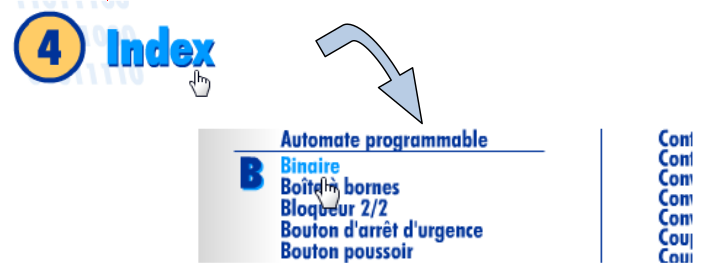
\includegraphics[width=.7\linewidth]{./figures/gda1.png}
\end{center}

Lire la présentation et répondez aux questions suivantes:
\begin{enumerate}
	\item Qu'appelle t'on TOR ? Préciser la nature de l'information.\\
\vspace{1em}
\begin{Form}
	\TextField[name=r1,width=\linewidth,height=2.5em,multiline=true]{}
\end{Form}
	\item Qu'est-ce qu'un Bit ? Qu'est-ce qu'un mot ?\\
\vspace{1em}
\begin{Form}
	\TextField[name=r2,width=\linewidth,height=2.5em,multiline=true]{}
\end{Form}
	\item Qu'appelle-t-on un octet ?\\
\vspace{1em}
\begin{Form}
	\TextField[name=r3,width=\linewidth,height=2.5em,multiline=true]{}
\end{Form}
	\item Que signifie, le bit de poids faible, le bit de poids fort, (MSB et LSB en anglais) ?\\
\vspace{1em}
\begin{Form}
	\TextField[name=r4,width=\linewidth,height=2.5em,multiline=true]{}
\end{Form}
	\item Définir simplement la base 2 (binaire) et la base 10 (décimale).\\
\vspace{1em}
\begin{Form}
	\TextField[name=r5,width=\linewidth,height=2.5em,multiline=true]{}
\end{Form}
	\item Décomposer le nombre décimal 425 en développant les chiffres significatifs, la base et le rang (le
		rang correspond à la position du chiffre significatif en partant de 0 et de la droite : le chiffre de l'unité
		est de rang 0 et le chiffre des dizaines est de rang 1).\\
\vspace{1em}
\begin{Form}
	\TextField[name=r6,width=\linewidth,height=2.5em,multiline=true]{}
\end{Form}
	\item Décomposer le nombre binaire 1101001 en développant les chiffres significatifs, la base et le rang.\\
\vspace{1em}
\begin{Form}
	\TextField[name=r7,width=\linewidth,height=2.5em,multiline=true]{}
\end{Form}
	\item Dans un octet combien peut-on coder de valeurs différentes ? Donner les nombres limites.\\
\vspace{1em}
\begin{Form}
	\TextField[name=r8,width=\linewidth,height=2.5em,multiline=true]{}
\end{Form}
	\item Quel unité utilise t'on en informatique pour exprimer une capacité de stockage ou de transfert.\\
\vspace{1em}
\begin{Form}
	\TextField[name=r9,width=\linewidth,height=2.5em,multiline=true]{}
\end{Form}
\begin{minipage}[b]{.08\linewidth}
	
\includegraphics[width=\linewidth]{./figures/info.png}
	\vspace{1em}
\end{minipage}
\hfill
\begin{minipage}[b]{.85\linewidth}
Pour distinguer l'écriture d'un nombre en binaire ou en décimal, nous adopterons la syntaxe suivante:
\begin{itemize}
	\item Le nombre N=(\texttt{101})$_{2}$ est un nombre écrit en binaire (indice 2 pour la base) qui vaut \textbf{cinq}.
	\item Le nombre N=(\texttt{101})$_{10}$ est un nombre écrit en décimal (indice 10 pour la base) qui vaut \textbf{cent un}.
\end{itemize}
\end{minipage}
	\item On souhaite connaître la valeur décimale (utilisée par l'homme) d'un nombre binaire (utilisé par la machine).
		Pour cela il faut convertir ce nombre binaire en nombre décimal.
		Toujours en vous aidant du GDA et en utilisant la méthode proposée, convertir les nombres binaires suivants en décimal (développer le résultat):\\
		\begin{itemize}
			\item \textbf{N1}=(\texttt{11011011})$_{2}$ = ( ? )$_{10}$\\
\vspace{1em}
\begin{Form}
	\TextField[name=r101,width=\linewidth,height=2.5em,multiline=true,default=N1=]{}
\end{Form}
			\item \textbf{N2}=(\texttt{11111001})$_{2}$ = ( ? )$_{10}$\\
\vspace{1em}
\begin{Form}
	\TextField[name=r102,width=\linewidth,height=2.5em,multiline=true,default=N2=]{}
\end{Form}
			\item \textbf{N3}=(\texttt{1100101001})$_{2}$ = ( ? )$_{10}$\\
\vspace{1em}
\begin{Form}
	\TextField[name=r102,width=\linewidth,height=2.5em,multiline=true,default=N3=]{}
\end{Form}
		\end{itemize}
	\item Convertir les nombres décimaux suivants en nombre binaire, faites-le en appliquant la méthode
		proposée puis vérifier votre résultat en utilisant l'outil de conversion du GDA, uniquement pour les
		deux premiers:
		\begin{itemize}
			\item \textbf{N4}=(\texttt{152})$_{10}$ = ( ? )$_{2}$\\
\vspace{1em}
\begin{Form}
	\TextField[name=r104,width=\linewidth,height=2.5em,multiline=true,default=N4=]{}
\end{Form}
			\item \textbf{N5}=(\texttt{270})$_{10}$ = ( ? )$_{2}$\\
\vspace{1em}
\begin{Form}
	\TextField[name=r105,width=\linewidth,height=2.5em,multiline=true,default=N5=]{}
\end{Form}
			\item \textbf{N6}=(\texttt{355})$_{10}$ = ( ? )$_{2}$\\
\vspace{1em}
\begin{Form}
	\TextField[name=r106,width=\linewidth,height=2.5em,multiline=true,default=N6=]{}
\end{Form}
			\item \textbf{N7}=(\texttt{504})$_{10}$ = ( ? )$_{2}$\\
\vspace{1em}
\begin{Form}
	\TextField[name=r107,width=\linewidth,height=2.5em,multiline=true,default=N7=]{}
\end{Form}
		\end{itemize}
\end{enumerate}

\section{La base Hexadécimale}
Dans le guide des automatismes, aller dans le chapitre \og{}index\fg{} et cliquer sur le mot \textbf{Hexadécimal}.

\begin{center}
	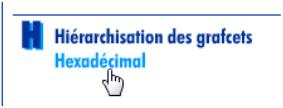
\includegraphics[width=.3\linewidth]{./figures/gda2.png}
\end{center}

\begin{enumerate}
	\setcounter{enumi}{11}
	\item Qu'appelle-t-on une base hexadécimale ? Dans quel but utilise-t-on l'hexadécimal ?\\
\vspace{1em}
\begin{Form}
	\TextField[name=r11,width=\linewidth,height=2.5em,multiline=true]{}
\end{Form}
	\item Compléter le tableau hexadécimal suivant:
\vspace{1em}
\begin{center}
	\begin{Form}
		\begin{tabular}{|c|c|c|c|c|c|}
			\hline
			Décimal & \multicolumn{4}{c|}{Binaire} & Héxadécimal \\
			\hline
			\hline
			0 & \TextField[name=r11b00,width=2em]{} & \TextField[name=r11b01,width=2em]{} & \TextField[name=r11b02,width=2em]{} & \TextField[name=r11b03,width=2em]{} & \TextField[name=r11h0,width=8em]{}\\
			\hline
			1 & \TextField[name=r11b10,width=2em]{} & \TextField[name=r11b11,width=2em]{} & \TextField[name=r11b12,width=2em]{} & \TextField[name=r11b13,width=2em]{} & \TextField[name=r11h1,width=8em]{}\\
			\hline
			2 & \TextField[name=r11b20,width=2em]{} & \TextField[name=r11b21,width=2em]{} & \TextField[name=r11b22,width=2em]{} & \TextField[name=r11b23,width=2em]{} & \TextField[name=r11h2,width=8em]{}\\
			\hline
			3 & \TextField[name=r11b30,width=2em]{} & \TextField[name=r11b31,width=2em]{} & \TextField[name=r11b32,width=2em]{} & \TextField[name=r11b33,width=2em]{} & \TextField[name=r11h3,width=8em]{}\\
			\hline
			4 & \TextField[name=r11b40,width=2em]{} & \TextField[name=r11b41,width=2em]{} & \TextField[name=r11b42,width=2em]{} & \TextField[name=r11b43,width=2em]{} & \TextField[name=r11h4,width=8em]{}\\
			\hline
			5 & \TextField[name=r11b50,width=2em]{} & \TextField[name=r11b51,width=2em]{} & \TextField[name=r11b52,width=2em]{} & \TextField[name=r11b53,width=2em]{} & \TextField[name=r11h5,width=8em]{}\\
			\hline
			6 & \TextField[name=r11b60,width=2em]{} & \TextField[name=r11b61,width=2em]{} & \TextField[name=r11b62,width=2em]{} & \TextField[name=r11b63,width=2em]{} & \TextField[name=r11h6,width=8em]{}\\
			\hline
			7 & \TextField[name=r11b70,width=2em]{} & \TextField[name=r11b71,width=2em]{} & \TextField[name=r11b72,width=2em]{} & \TextField[name=r11b73,width=2em]{} & \TextField[name=r11h7,width=8em]{}\\
			\hline
			8 & \TextField[name=r11b80,width=2em]{} & \TextField[name=r11b81,width=2em]{} & \TextField[name=r11b82,width=2em]{} & \TextField[name=r11b83,width=2em]{} & \TextField[name=r11h8,width=8em]{}\\
			\hline
			9 & \TextField[name=r11b90,width=2em]{} & \TextField[name=r11b91,width=2em]{} & \TextField[name=r11b92,width=2em]{} & \TextField[name=r11b93,width=2em]{} & \TextField[name=r11h9,width=8em]{}\\
			\hline
			10 & \TextField[name=r11bA0,width=2em]{} & \TextField[name=r11bA1,width=2em]{} & \TextField[name=r11bA2,width=2em]{} & \TextField[name=r11bA3,width=2em]{} & \TextField[name=r11hA,width=8em]{}\\
			\hline
			11 & \TextField[name=r11bB0,width=2em]{} & \TextField[name=r11bB1,width=2em]{} & \TextField[name=r11bB2,width=2em]{} & \TextField[name=r11bB3,width=2em]{} & \TextField[name=r11hB,width=8em]{}\\
			\hline
			12 & \TextField[name=r11bC0,width=2em]{} & \TextField[name=r11bC1,width=2em]{} & \TextField[name=r11bC2,width=2em]{} & \TextField[name=r11bC3,width=2em]{} & \TextField[name=r11hC,width=8em]{}\\
			\hline
			13 & \TextField[name=r11bD0,width=2em]{} & \TextField[name=r11bD1,width=2em]{} & \TextField[name=r11bD2,width=2em]{} & \TextField[name=r11bD3,width=2em]{} & \TextField[name=r11hD,width=8em]{}\\
			\hline
			14 & \TextField[name=r11bE0,width=2em]{} & \TextField[name=r11bE1,width=2em]{} & \TextField[name=r11bE2,width=2em]{} & \TextField[name=r11bE3,width=2em]{} & \TextField[name=r11hE,width=8em]{}\\
			\hline
			15 & \TextField[name=r11bF0,width=2em]{} & \TextField[name=r11bF1,width=2em]{} & \TextField[name=r11bF2,width=2em]{} & \TextField[name=r11bF3,width=2em]{} & \TextField[name=r11hF,width=8em]{}\\
			\hline
		\end{tabular}
	\end{Form}
\end{center}

\vspace{2em}
\begin{minipage}[b]{.08\linewidth}
	
\includegraphics[width=\linewidth]{./figures/info.png}
%	\vspace{1em}
\end{minipage}
\hfill
\begin{minipage}[b]{.85\linewidth}
Pour désigner un nombre hexadécimal nous adopterons la syntaxe suivante:\\

Le nombre N=(\texttt{101})$_{16}$ est un nombre écrit hexadécimal (indice 16 pour la base) et qui vaut deux cent cinquante-sept.
\end{minipage}

	\item Convertir les nombres suivants dans la base souhaitée, faites-le en appliquant la méthode proposée
		puis vérifier votre résultat en utilisant l'outil de conversion du GDA, uniquement pour les quatre premiers.
		\begin{itemize}
			\item \textbf{N8}=(\texttt{11010111})$_{2}$ = ( ? )$_{16}$\\
\vspace{1em}
\begin{Form}
	\TextField[name=r148,width=\linewidth,height=2.5em,multiline=true,default=N8=]{}
\end{Form}
			\item \textbf{N9} = (\texttt{01010001})$_{2}$ = ( ? )$_{16}$\\
\vspace{1em}
\begin{Form}
	\TextField[name=r148,width=\linewidth,height=2.5em,multiline=true,default=N9=]{}
\end{Form}
			\item \textbf{N10} = (\texttt{A5})$_{16}$ = ( ? )$_{2}$\\
\vspace{1em}
\begin{Form}
	\TextField[name=r148,width=\linewidth,height=2.5em,multiline=true,default=N10=]{}
\end{Form}
			\item \textbf{N11} = (\texttt{F9})$_{16}$  = ( ? )$_{2}$\\
\vspace{1em}
\begin{Form}
	\TextField[name=r148,width=\linewidth,height=2.5em,multiline=true,default=N11=]{}
\end{Form}
			\item \textbf{N12} = (\texttt{11110010001})$_{2}$ = ( ? )$_{16}$\\
\vspace{1em}
\begin{Form}
	\TextField[name=r148,width=\linewidth,height=2.5em,multiline=true,default=N12=]{}
\end{Form}
			\item \textbf{N13} = (\texttt{DFE})$_{16}$ = ( ? )$_{2}$\\
\vspace{1em}
\begin{Form}
	\TextField[name=r148,width=\linewidth,height=2.5em,multiline=true,default=N13=]{}
\end{Form}
		\end{itemize}

	\item Compléter le tableau suivant, pour une valeur donnée indiquer les valeurs manquantes.
\begin{center}
	\begin{Form}
		\begin{tabular}{|c|c|c|}
			\hline
			Binaire & Héxadécimal & Décimal \\
			\hline
			\hline
			\TextField[name=r15b0,width=8em]{} & \TextField[name=r15h0,width=4em]{} & \texttt{315}\\
			\hline
			\texttt{1011011101} & \TextField[name=r15h1,width=4em]{} & \TextField[name=r15d1,width=4em]{}\\
			\hline
			\TextField[name=r15b2,width=8em]{} & \texttt{F9DE} & \TextField[name=r15d2,width=4em]{}\\
			\hline
		\end{tabular}
	\end{Form}
\end{center}
\end{enumerate}

\section{Le code DCB ou BCD}
Dans le guide des automatismes, aller dans le chapitre \og{}Index\fg{} et cliquer sur le terme \textbf{Code BCD / DCB}.

\begin{center}
	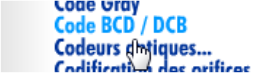
\includegraphics[width=.3\linewidth]{./figures/gda3.png}
\end{center}

\begin{enumerate}
	\setcounter{enumi}{15}
	\item Que signifie DCB (ou BCD en anglais) ?\\
\vspace{1em}
\begin{Form}
	\TextField[name=r16,width=\linewidth,height=2.5em,multiline=true]{}
\end{Form}

\begin{minipage}[b]{.08\linewidth}
	
\includegraphics[width=\linewidth]{./figures/info.png}
\end{minipage}
\hfill
\begin{minipage}[b]{.85\linewidth}
	Pour désigner un nombre BCD, nous adopterons la syntaxe suivante:\\

	Le nombre N=(\texttt{1001 0100})$_{BCD}$ est un nombre écrit en BCD et qui vaut quatre-vingt-quatorze.
\end{minipage}
	\item Convertir les nombres suivants dans la base spécifiée:
		\begin{itemize}
			\item \textbf{N14}=(\texttt{18})$_{10}$ = ( ? )$_{BCD}$\\
\vspace{1em}
\begin{Form}
	\TextField[name=r1714,width=\linewidth,height=2.5em,multiline=true,default=N14=]{}
\end{Form}
			\item \textbf{N15}=(\texttt{9203})$_{10}$ = ( ? )$_{BCD}$\\
\vspace{1em}
\begin{Form}
	\TextField[name=r1715,width=\linewidth,height=2.5em,multiline=true,default=N15=]{}
\end{Form}
			\item \textbf{N16}=(\texttt{001110010001})$_{BCD}$ = ( ? )$_{10}$\\
\vspace{1em}
\begin{Form}
	\TextField[name=r1716,width=\linewidth,height=2.5em,multiline=true,default=N16=]{}
\end{Form}
			\item \textbf{N17}=(\texttt{0111 1000 0110 0010})$_{BCD}$ = ( ? )$_{10}$\\
\vspace{1em}
\begin{Form}
	\TextField[name=r1717,width=\linewidth,height=2.5em,multiline=true,default=N17=]{}
\end{Form}
		\end{itemize}
\end{enumerate}
\section{Le code ASCII}
Le \textbf{code ASCII} (\emph{American Standard Code for Information Interchange}) \textbf{est un code alphanumérique} universel utilisé dans
presque tous les ordinateurs. La plupart des claviers d'ordinateurs utilisent une norme basée sur le code ACSII : à
chaque entrée de lettre, de chiffre ou d'une commande, le code numérique correspondant est dirigé vers l'unité centrale.

Le code ASCII d'un caractère est le nombre qui lui est associé (ce code attribue les valeurs 0 à 255 aux différents caractères).

Le \textbf{code ASCII standard} (de 0 à 127) permet de représenter les \textbf{128 caractères de base}. 
Les 32 premiers caractères sont des caractères de contrôle (ex : changement de ligne, retour chariot...) ;
les caractères suivants sont les lettres minuscules et majuscules, les chiffres et les signes de ponctuation.

Le \textbf{code ASCII étendu} (de 128 à 255) permet de représenter les \textbf{128 caractères additionnels} : caractères alphabétiques
étrangers, symboles mathématiques et caractères de dessin.

\textbf{Tableau représentant la liste du code ASCII à 7 bits :}

\textbf{Exemple de lecture du tableau :} la lettre \textbf{B} est représentée par le groupe codé de b0 à b3 (code ligne) et de b4 à b6
(code colonne) : \textbf{B $\Rightarrow$ \color{red}1000010} en binaire soit \textbf{\color{red}66} en décimal et \textbf{\color{red}42} en hexadécimal.

\begin{center}
	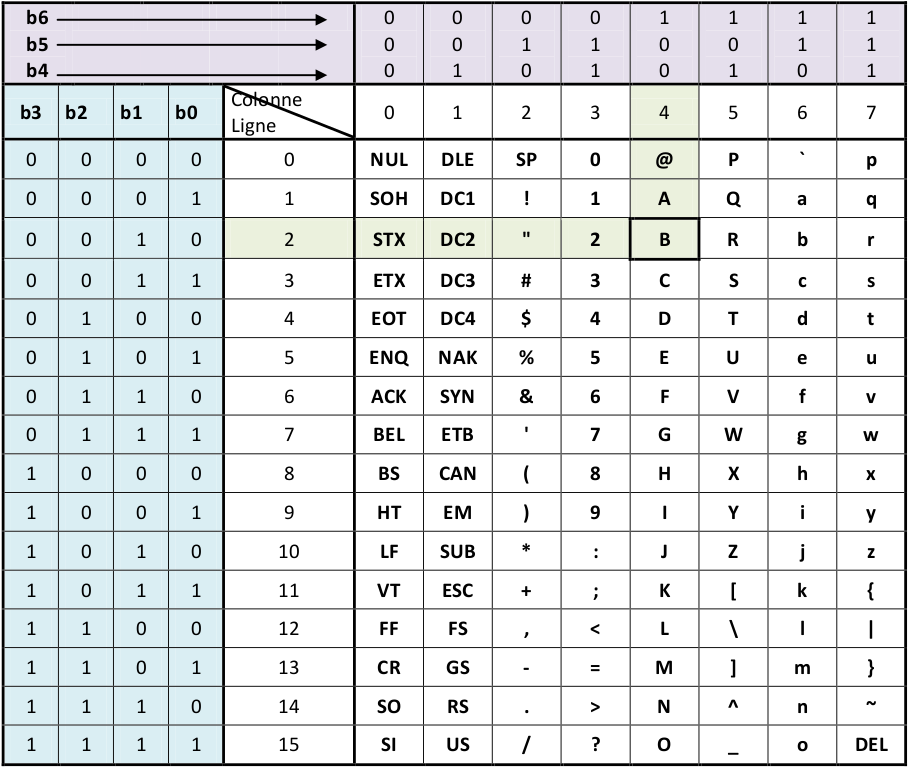
\includegraphics[scale=.6]{./figures/ascii1.png}
\end{center}
\paragraph{Description des codes spéciaux :}
\begin{center}
	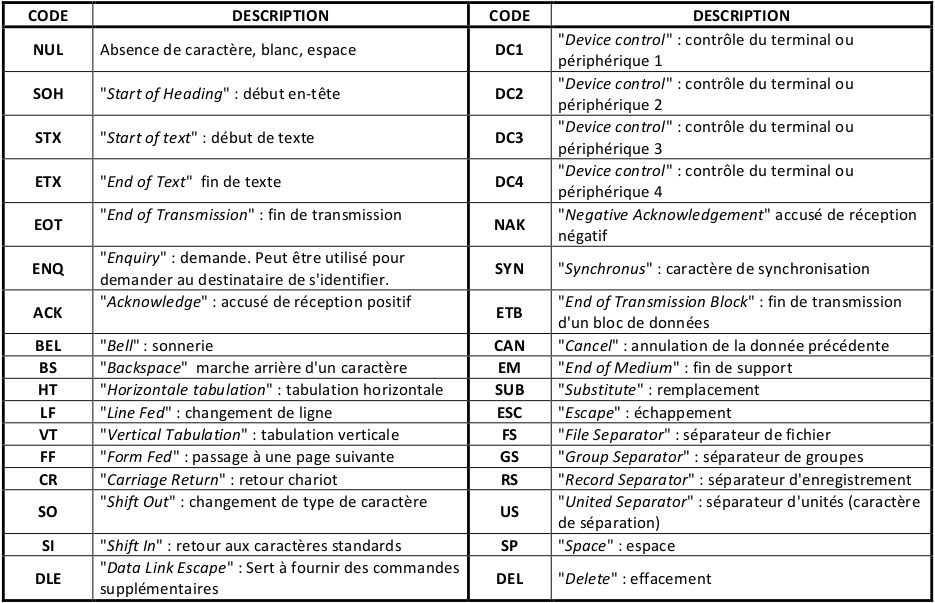
\includegraphics[scale=.6]{./figures/ascii2.png}
\end{center}
\paragraph{Tableau représentant la liste du code ASCII à 8 bits (code ASCII étendu) :\\}
Les combinaisons de 80 à FF sont à usage strictement national. Ainsi pour ces 128 dernières combinaisons, on trouve
pour la France les caractères (î, è, à, etc.). Par exemple le caractère â est codé en hexadécimal (83) 16 .
\begin{center}
	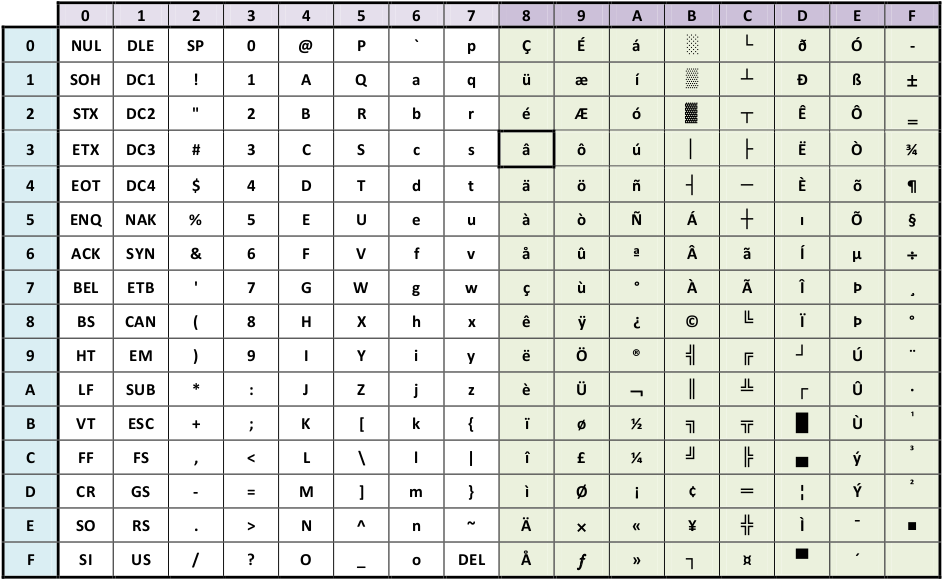
\includegraphics[scale=.6]{./figures/ascii3.png}
\end{center}
\begin{enumerate}
	\setcounter{enumi}{17}
	\item Quelle est l'utilité du code ASCII ?\\
\vspace{1em}
\begin{Form}
	\TextField[name=r18,width=\linewidth,height=2.5em,multiline=true]{}
\end{Form}
	\item Donner le code décimal, Hexadécimal et binaire des caractères contenus dans le tableau suivant pour un code ASCII 8 bits.
\begin{center}
	\begin{Form}
		\begin{tabular}{|c|c|c|c|}
			\hline
			Caractère & Décimal & Hexadécimal & Binaire\\
			\hline
			\hline
			W & \TextField[name=r19d1,width=4em]{} & \TextField[name=r19h1,width=3em]{} & \TextField[name=r19b1,width=8em]{}\\
			\hline
			m & \TextField[name=r19d2,width=4em]{} & \TextField[name=r19h2,width=3em]{} & \TextField[name=r19b2,width=8em]{}\\
			\hline
			2 & \TextField[name=r19d3,width=4em]{} & \TextField[name=r19h3,width=3em]{} & \TextField[name=r19b3,width=8em]{}\\
			\hline
		\end{tabular}
	\end{Form}
\end{center}
	\item La séquence de bits \textbf{\color{red}1010000100000110001100100001} est une chaîne de caractères ASCII 7 bits.
		Décoder cette chaîne.\\
\vspace{1em}
\begin{Form}
	\TextField[name=r20,width=\linewidth,height=2.5em,multiline=true]{}
\end{Form}
	\item Notez votre prénom sous forme d'une chaîne de carcatères, puis son code ASCII 8-bit en hexadécimal.\\
\begin{Form}
	\TextField[name=r21,width=\linewidth,height=2.5em,multiline=true]{}
\end{Form}
\end{enumerate}
\end{document}
